\tikzstyle{goal} = [draw, rectangle, minimum width=1cm, minimum height=2em, very thick, rounded corners=1mm]
\tikzstyle{ded}  = [-stealth,very thick]
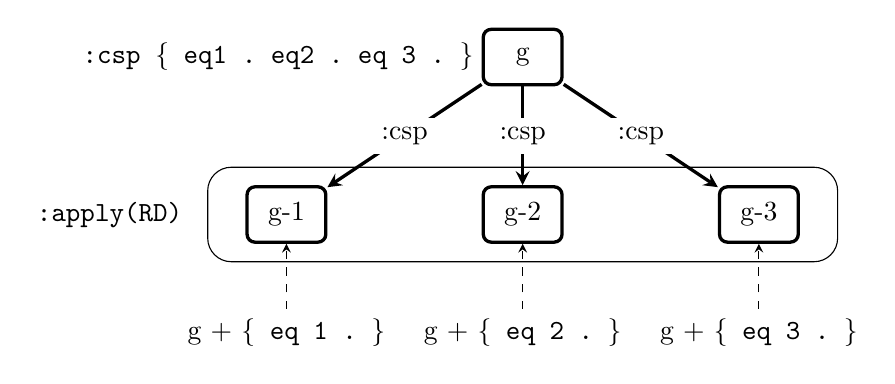
\begin{tikzpicture}[node distance=3cm]
  \node at (0,4) (g) [goal] {g};
  \node at (-3,2) (g-1)   [goal] {g-1};
  \node at (0,2)  (g-2)   [goal] {g-2};
  \node at (3,2) (g-3)   [goal] {g-3};
  \node [left of=g,node distance=0.5cm,anchor=east] 
    {\texttt{\texttt{:csp \{ eq1 .\ eq2 .\ eq 3 .\ \}}}};
  \draw[rounded corners=3mm] (-4,1.4) rectangle (4,2.6);
  \path[ded] (g) edge node[fill=white] {:csp} (g-1)
                 edge node[fill=white] {:csp} (g-2)
                 edge node[fill=white] {:csp} (g-3) ;
  \node at (-3,0.5) (a1) {g + \texttt{\{ eq 1\ .\ \}}} ;
  \node at ( 0,0.5) (a2) {g + \texttt{\{ eq 2\ .\ \}}} ;
  \node at ( 3,0.5) (a3) {g + \texttt{\{ eq 3\ .\ \}}} ;
  \path[-stealth,dashed] (a1) edge (g-1) ;
  \path[-stealth,dashed] (a2) edge (g-2) ;
  \path[-stealth,dashed] (a3) edge (g-3) ;
  \node at (-4.2,2) [anchor=east] {\texttt{:apply(RD)}} ;
\end{tikzpicture}
